\documentclass[12pt,a4paper, spanish]{report}
\usepackage[spanish]{babel}
\usepackage[latin1]{inputenc}  % Ambos para solucin de asuntos de idioma
\usepackage[T1]{fontenc}
\usepackage{tocbibind}  % Bibliografa en el indice
\usepackage{titlesec}  % Posibilidad de editar los formatos de chapter y section
%\usepackage{times}  % Fuente de letras
\usepackage{amsmath,amssymb,mathrsfs,mathptmx}  % Matemticas varias
\usepackage{hyperref} % Para escribir URLs
\usepackage[vlined,ruled]{algorithm2e}


% --- Arreglos varios para la inclusion de imgenes
%\usepackage[pdftex]{graphicx}
%\usepackage[dvips]{graphicx}
\usepackage{graphicx}
\usepackage{epsfig}

\usepackage{float}
\usepackage{subfigure}
%\usepackage{subfig}
\usepackage{wrapfig}
\usepackage[usenames,dvipsnames]{color}
\DeclareGraphicsExtensions{.png,.jpg,.pdf,.mps,.gif,.bmp, .eps}


\usepackage{multirow}
\usepackage{multicol}
\usepackage{tabulary}
\usepackage[table]{xcolor}
\usepackage{color}
\usepackage{listings}
%\usepackage{subfloat}
\usepackage{tikz}

\setcounter{secnumdepth}{3}
\setcounter{tocdepth}{3}


% --- Para las dimensiones de los mrgenes etc
\frenchspacing \addtolength{\hoffset}{-1.5cm}
\addtolength{\textwidth}{3cm} \addtolength{\voffset}{-2.5cm}
\addtolength{\textheight}{4cm}
% --- Para el encabezado
\usepackage{fancyhdr}
\fancyhead[R]{2012}\fancyhead[L]{enCuadro} \fancyfoot[C]{\thepage}
\pagestyle{fancy}

% --- Formato de la etiqueta Chapter
%\newcommand{\bigrule}{\titlerule[0.5mm]}
%\titleformat{\chapter}[display]{\bfseries\Huge}
%{\Large\chaptertitlename\ \Large\thechapter}
%{0mm} {\filleft} [\vspace{0.5mm} \bigrule]

\titleformat{\chapter}[display]
{\normalfont\Large\filcenter}
{\titlerule[1pt]%
\vspace{1pt}%
\titlerule
\vspace{1pc}%
\LARGE\MakeUppercase{\chaptertitlename} \thechapter}
{1pc}
{\titlerule
\vspace{1pc}%
\Huge}

%-------------------------

\begin{document}
% Esto es para que se muestren todas las referencias aunque no se citen:
\nocite{*}

\renewcommand{\tablename}{Tabla}
\renewcommand{\theenumi}{\Roman{enumi}}
\renewcommand{\labelenumi}{[\textbf{\theenumi}]}
\renewcommand{\thefootnote}{\arabic{footnote}}
% --- Modificacin de entornos enumerate
\renewcommand{\theenumi}{\roman{enumi}}
\renewcommand{\labelenumi}{\theenumi)}
% --- Modificacin de entornos enumerate

% --- Para hacer highlights
\newcommand{\highlAmarillo}[1]{\colorbox{yellow}{#1}}
\newcommand{\highlVerde}[1]{\colorbox{green}{#1}}
\newcommand{\highlRojo}[1]{\colorbox{red}{#1}}

%

\begin{titlepage}

\vskip2.5cm
\begin{center}
\begin{tabular}{p{1cm} p{11cm}  p{1cm}}
 &
\large{
\begin{center}
\sc Proyecto de fin de estudios \\
\sc en la carrera Ingenier�a El�ctrica\\
\end{center}
} &
\end{tabular}
\end{center}

%\begin{picture}(0,0)
%\put(-35,20){\includegraphics[width=5cm]{Imagenes/logo_udelar.eps}}
%\end{picture}

%\begin{picture}(0,0)
%\put(338,35){\includegraphics[width=5cm]{Imagenes/logo_udelar.eps}}
%\end{picture}

\vskip3cm

\begin{center}
\Huge {\textbf{encuadro}}\\
\Large {Aplicaci�n de realidad aumentada y navegaci�n para museos sobre dispositivos m�viles}
\end{center}

\vskip2cm

\begin{center}
\Large {\sc \textbf{Documentaci�n Final}}\\
\Large {\sc \textbf{A\~no 2012}}\\
\end{center}

\vskip2cm

%\begin{center}
%\Large {\textbf{CubeSatET} es parte del \textbf{Proyecto LAI}}\\
%\end{center}

\vskip3cm

\begin{flushright}
\begin{tabular}{r l}
\large{\underline{\bf Tutor:}}\vspace{0.2cm}\\
\large{\textbf{Juan Cardelino}}\\
\end{tabular}
\end{flushright}

\vskip1cm

\begin{flushright}
\begin{tabular}{r l}
\large{\underline{\bf Integrantes:}}\vspace{0.2cm}\\
\large{\textbf{Juan Braun}}\\
juanibraun@gmail.com\\
\large{\textbf{Mart�n Etchart}}\\
mrtn.etchart@gmail.com\\
\large{\textbf{Pablo Flores}}\\
pablofloresguridi@gmail.com\\
\large{\textbf{Mauricio Gonz�lez}}\\
mgonzaleznappa@gmail.com\\
\end{tabular}
\end{flushright}


\end{titlepage}

\tableofcontents

\chapter{Modelo de c�mara y estimaci�n de pose monocular}
\label{chap: camypose}
% !TEX encoding = IsoLatin

%Definici�n de realidad aumentada, ejemplos. Breve menci�n de las cosas que se usan, modelo c�mara pinhole, calibraci�n, extracci�n de caracter�sticas(LSD,ORT), marcador utilizado.
%Algoritmos de estimaci�n de pose. Algoritmos de correspondencias. Toda la rama Posit
%Habria que hacer un diagrama de bloques que muestre el flujo para hallar la pose

\section{Introducci�n}
% ------------------------------------------------------ INTRODUCCION: DEFINICION DE ESTIMACION DE POSE -------------------------------------------------------

Se le llama ``estimaci�n de pose'' al proceso mediente el cual se calcula en qu� punto del mundo y con qu� orientaci�n se encuentra determinado objeto respecto de un eje de coordenadas previamente definido al que se lo llama ``ejes del mundo''. Las aplicaciones de realidad aumentada requieren de un modelado preciso del entorno respecto de estos ejes, para poder ubicar correctamente los agregados virtuales dentro del modelo y luego dibujarlos de forma coherente en la imagen vista por el usuario. El objeto cuya estimaci�n de pose resulta de mayor importancia es la c�mara, ya que por �sta es por donde se mira la escena y es respecto de �sta que los objetos virtuales deben ubicarse de manera consistente.  Una forma de estimar la pose de la c�mara es mediante el uso de las im�genes capturadas por ella misma.  Asimismo, el concepto ``monocular'' hace referencia al uso de una sola c�mara, ya que es posible trabajar con m�s de una.

Para poder obtener informaci�n relevante a partir de las im�genes tomadas por una c�mara, resulta necesario contar con un modelo preciso de su arquitectura ya que no todas las c�maras son iguales. El modelo m�s comunmente utilizado es el denominado \textit{pin-hole}. Para modelar completamente la arquitectura de la c�mara se deben estimar ciertos ``par�metros intr�nsecos'' a �sta, y eso se logra luego de realizados ciertos experimentos. A la estimaci�n de estos par�metros se le denomina ``calibraci�n de la c�mara''.

En este cap�tulo se ver� en detalle el modelo de c�mara \textit{pin-hole}, tomando en cuenta la distorsi�n introducida por las lentes. M�s adelante, se mencionar�n distintos m�todos para la calibraci�n de una c�mara y se ver� en detalle en particular, el m�todo de Zhang. 

Tambi�n se presentan los algoritmos m�s utilizados para el problema de estimaci�n de pose, entre ellos el DLT(Direct Linear Transform), P\textit{n}P(Perspective \textit{n} Point) y RANSAC(RANdom SAmple Consensus).

Finalmente se presentan las diferentes maneras que hay para representar los �ngulos de la pose y los problemas que se presentan cuando se trabaja con estas representaciones. 
%\begin{figure}[h]
%\centering
%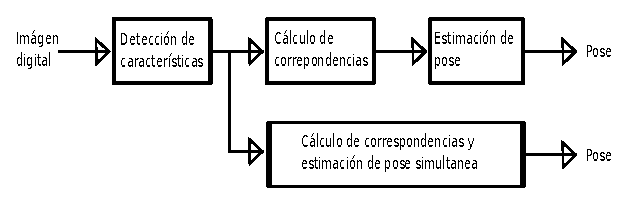
\includegraphics[scale=1.5]{../imagenes/EstPose/EstPose_1.eps}
%\caption{Diagrama de bloques para el proceso de estimaci�n de pose.}
%\label{EstPose_1}
%\end{figure}
%En este cap�tulo se presentan las t�cnicas realizadas para implementar la realidad aumentada

% ------------------------------------------------------ CALIBRACION DE CAMARA: MODELO PIN-HOLE -------------------------------------------------------
\section{Modelo de c�mara \textit{pin-hole} \cite{garciaocon07}}
\label{sec:Calibracion de camara}


\subsection{Fundamentos y definiciones}
\label{sec:Fundamentos y definiciones}
Este modelo consiste en un centro �ptico O, en donde convergen todos los rayos de la proyecci�n y un plano imagen en el cual la imagen es proyectada. Se define \textit{distancia focal} ($f$) como la distancia entre el centro �ptico O y la intersecci�n del eje �ptico con el plano imagen (punto C). Ver Figura \ref{fig:CalibracionCamara}.  

\begin{figure}[h!]
\centering
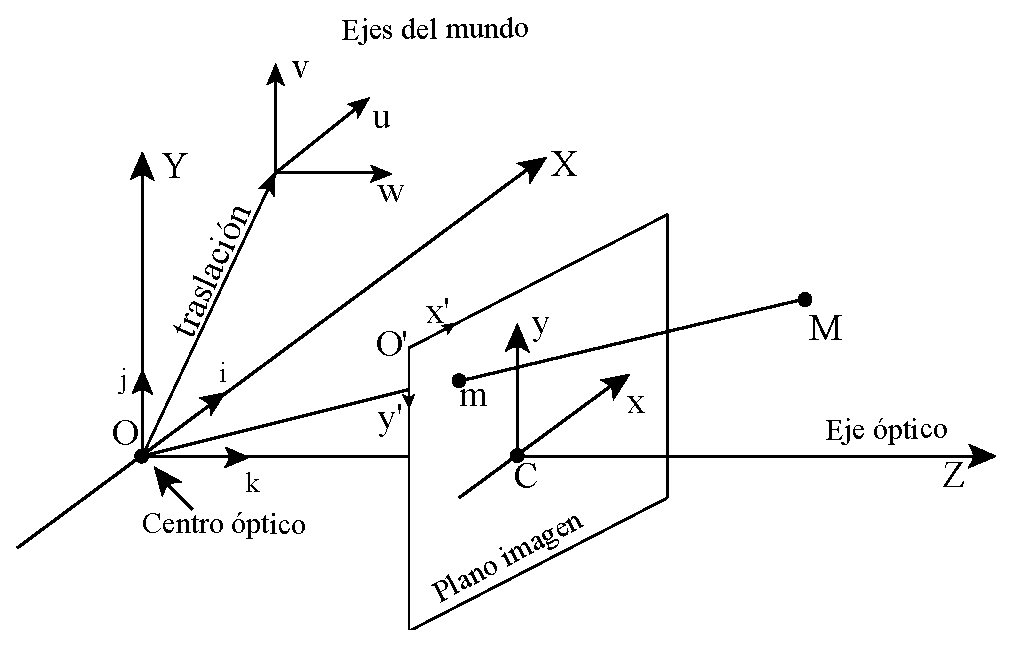
\includegraphics[scale=0.8]{figs_camaraypose/CalibracionCamara.eps}
\caption{Modelo de c�mara pin-hole.}
\label{fig:CalibracionCamara}
\end{figure}

Se llama proceso de pryecci�n al proceso en el que se asocia al punto \textbf{M} del mundo, un punto \textbf{m} en la imagen. Para modelar el mismo es necesario referirse a varias transformaciones y varios ejes de coordenadas.
\begin{itemize}
\item \textit{Coordenadas del mundo}: son las coordenadas que describen la posici�n 3D del punto \textbf{M} respecto de los ejes del mundo $(u,v,w)$. La elecci�n de los ejes del mundo es arbitraria.
\item \textit{Coordenadas de la c�mara}: son las coordenadas que describen la posici�n del punto \textbf{M} respecto de los ejes de la c�mara $(X,Y,Z)$. $i$, $j$ y $k$ son los versores de este eje de coordenadas.
\item \textit{Coordenadas de la imagen}: son las coordenadas que describen la posici�n del punto 2D, \textbf{m} respecto del centro del plano imagen, C. Los ejes de este sistema de coordenadas son $(x,y)$.
\item \textit{Coordenadas normalizadas de la imagen}: son las coordenadas que describen la posici�n del punto 2D, \textbf{m}, respecto del eje de coordenadas $(x',y')$ situado en la esquina superior izquierda del plano imagen.
\end{itemize}
La transformaci�n que lleva al punto \textbf{M}, expresado respecto de los ejes del mundo, al punto \textbf{m}, expresado respecto del sistema de coordenadas normalizadas de la imagen, se puede ver como la composici�n de dos transformaciones menores. La primera, es la que realiza la proyecci�n que transforma a un punto definido respecto del sistema de coordenadas de la c�mara $(X, Y, Z)$ en otro punto sobre el plano imagen expresado respecto del sistema de coordenadas normalizadas de la imagen $(x',y')$. V�ase que una vez calculada esta transformaci�n, es una constante caracter�stica de cada c�mara. Al conjunto de valores que definen esta transformaci�n, se le llama ``{par�metros intr�nsecos'' de la c�mara. La segunda, es la transformaci�n que lleva de expresar un punto respecto de los ejes del mundo $(u,v,w)$, a ser expresado seg�n los ejes de la c�mara $(X ,Y, Z)$. Esta �ltima transformaci�n var�a conforme se mueve la c�mara (respecto de los ejes del mundo) y el conjunto de valores que la definen es denominado ``par�metros extr�nsecos'' de la c�mara. Del c�lculo de estos par�metros es que se obtiene la estimaci�n de la pose de la c�mara.\\
De lo anterior se concluye r�pidamente que si se le llama $H$ a la matriz proyecci�n total, tal que:
\[
m = H.M,
\]
entonces:
\[
H = I.E
\]
donde $I$ corresponde a la matriz proyecci�n asociada a los par�metros intr�nsecos y $E$ corresponde a la matriz asociada a los par�metros extr�nsecos. Ambos juegos de par�metros acarrean informaci�n muy valiosa:  \\

\begin{itemize}
\item \textbf{Par�metros extr�nsecos:} pose de la c�mara.
\begin{itemize}
\item \underline{Traslaci�n:} ubicaci�n del centro �ptico de la c�mara respecto de los ejes del mundo.
\item \underline{Rotaci�n:} rotaci�n del sistema de coordenadas de la c�mara $(X ,Y, Z)$, respecto de los ejes del mundo.
\end{itemize}
\item \textbf{Par�metros intr�nsecos:} par�metros propios de la c�mara. Dependen de su geometr�a interna y de su �ptica.
\begin{itemize}
\item \underline{Punto principal (C = [$x'_C,y'_C$]):} es el punto intersecci�n entre el eje �ptico y el plano imagen. Las coordenadas de este punto vienen dadas en p�xeles y son expresadas respecto del sistema normalizado de la imagen.
\item \underline{Factores de conversi�n p�xel-mil�metros ($d_x,d_y$):} indican el n�mero de p�xeles por mil�metro que utiliza la c�mara en las direcciones $x$ e $y$ respectivamente.
\item \underline{Distancia focal (f):} distancia entre el centro �ptico (\textbf{O}) y el punto principal (\textbf{C}). Su unidad es el mil�metro.
\item \underline{Factor de proporci�n (s):} indica la proporci�n entre las dimensiones horizontal y vertical de un p�xel.   
\end{itemize}
\end{itemize}


\subsection{Matriz de proyecci�n}
\label{sec:Matriz de proyecci�n}

En la secci�n anterior se vio que es posible hallar una ``matriz de proyecci�n'' H que dependa tanto de los par�metros intr�nsecos de la c�mara como de sus par�metros extr�nsecos:
\[
m = H.M
\] 
donde \textbf{M} y \textbf{m} son los puntos ya definidos y vienen expresados en ``coordenadas homog�neas''. Por m�s informaci�n acerca de este tipo de coordenadas ver \cite{Hartley2004}.\\
Para determinar la forma de la matriz de proyecci�n se estudia c�mo se relacionan las coordenadas de \textbf{M} con las coordenads de \textbf{m}; para hallar esta relaci�n se debe analizar cada transformaci�n, entre los sistemas de coordenadas mencionados con anterioridad, por separado.\\
\begin{itemize}
\item \textbf{Proyecci�n 3D - 2D:} de las coordenadas homog�neas del punto \textbf{M} expresadas en el sistema de coordenadas de la c�mara $(X_0,Y_0,Z_0,T_0)$, a las coordenadas homog�neas del punto \textbf{m} expresadas en el sistema de coordenadas de la imagen $(x_0,y_0,s_0)$:\\
Se desprende de la imagen \ref{fig:CalibracionCamara} y algo de trigonometr�a la siguiente relaci�n entre las coordenadas en cuesti�n y la distancia focal (f):
\[
\frac{f}{Z_0} = \frac{x_0}{X_0} = \frac{y_0}{Y_0}
\]
A partir de la relaci�n anterior:
\[
\left( \begin{array}{c}
x_0 \\
y_0
\end{array} \right)
=
\frac{f}{Z_0} 
\left( \begin{array}{c}
X_0 \\ 
Y_0
\end{array} \right)
\]
Expresado en forma matricial, en coordenadas homog�neas:
\[
\left( \begin{array}{c}
x_0 \\
y_0 \\
s_0
\end{array} \right)
= 
\left( \begin{array}{cccc}
f & 0 & 0 & 0 \\ 
0 & f & 0 & 0 \\
0 & 0 & 1 & 0
\end{array} \right)
\left( \begin{array}{c}
X_0 \\ 
Y_0 \\
Z_0 \\
1
\end{array} \right)
\]
\item \textbf{Transformaci�n imagen - imagen:} de las coordenadas homog�neas del punto \textbf{m} expresadas respecto del sistema de coordenadas de la imagen $(x_0,y_0,s_0)$, a las coordenadas homog�neas de �l mismo pero expresadas respecto del sistema de coordenadas normalizadas de la imagen $(x'_0,y'_0,s'_0)$:\\

\begin{figure}[h!]
\centering
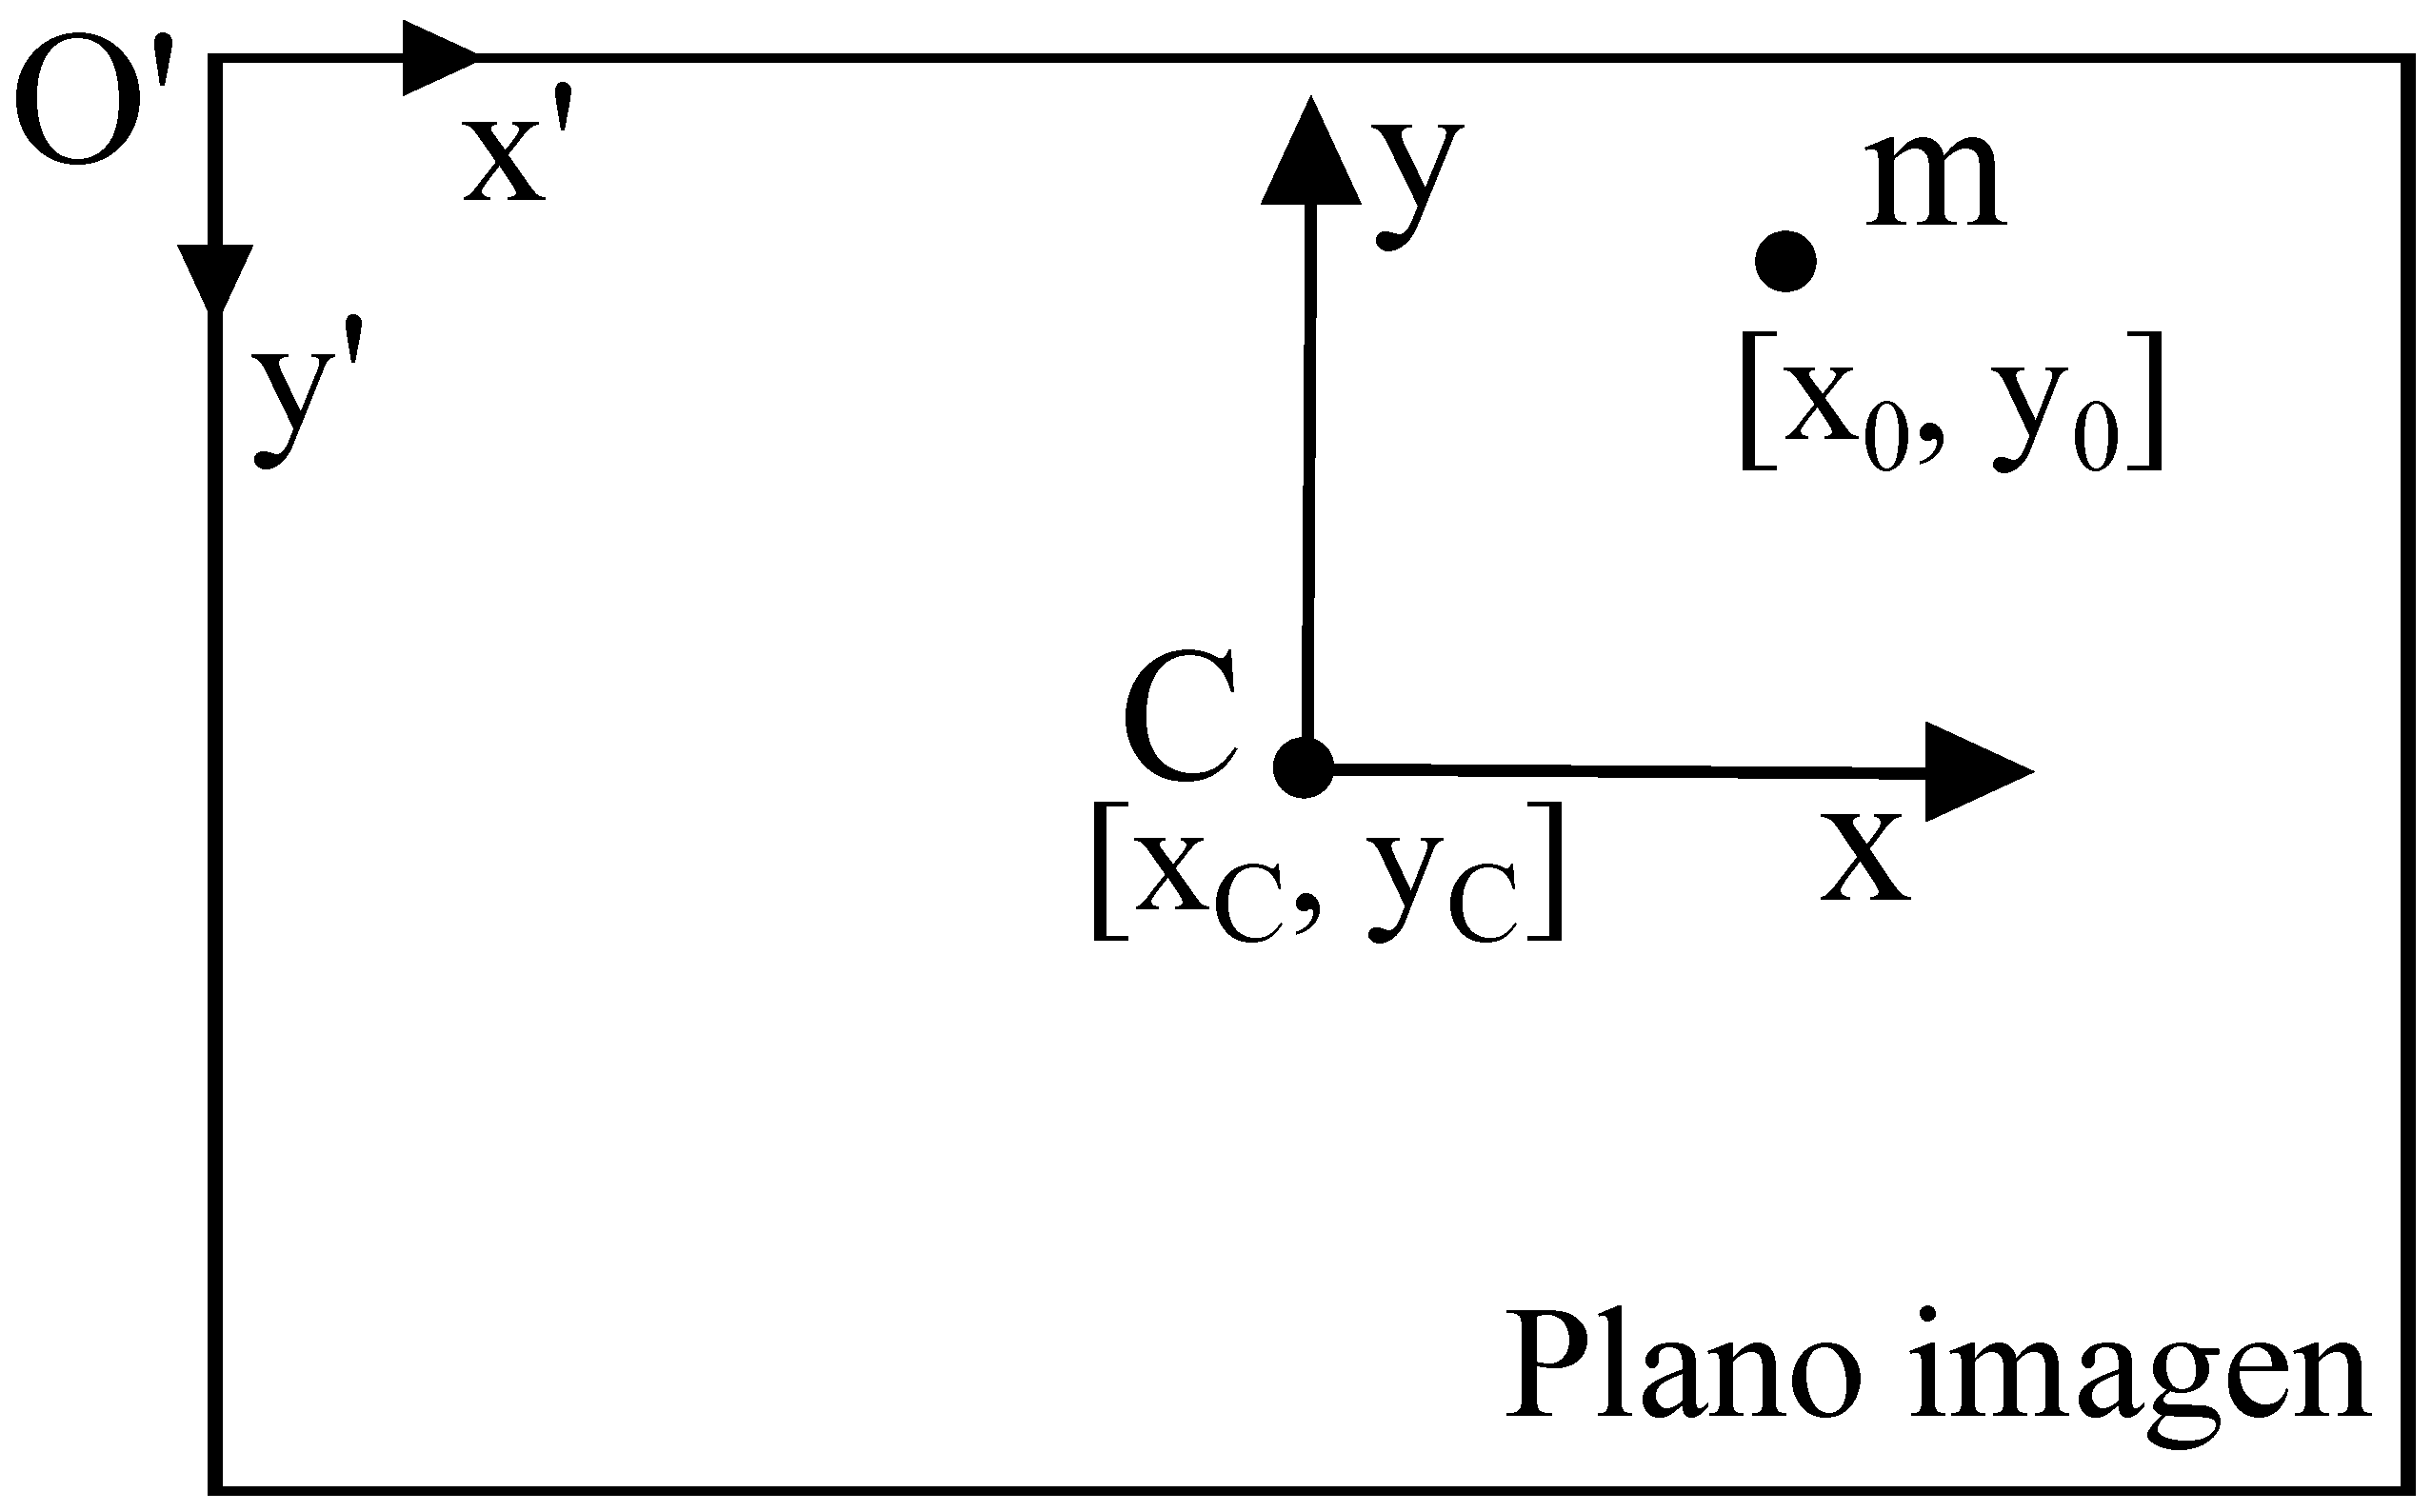
\includegraphics[scale=0.2]{figs_camaraypose/ParametrosIntrinsecos.eps}
\caption{Relaci�n entre el sistema de coordenadas de la imagen y el sistema de coordenandas normalizadas de la imagen.}
\label{fig:ParametrosIntrinsecos}
\end{figure}


Se les suma, a las coordenadas de \textbf{m} respecto del sistema de la imagen, la posici�n del punto C respecto del sistema normalizado de la imagen $(x'_C,y'_C)$. Las coordenadas de \textbf{m} dejan de ser expresadas en mil�metros para ser expresadas en p�xeles. Aparecen los factores de conversi�n $d_x$ y $d_y$:
\[
\begin{array}{c}
x'_0 = d_x.x_0 + x'_C \\
y'_0 = d_y.y_0 + y'_C
\end{array}
\]
Se obtiene entonces la siguiente relaci�n matricial, en coordenadas homog�neas:
\[
\left( \begin{array}{c}
x'_0 \\
y'_0 \\
s'_0
\end{array} \right)
= 
\left( \begin{array}{ccc}
d_x & 0 & x'_C \\ 
0 & d_y & y'_C \\
0 & 0 & 1
\end{array} \right)
\left( \begin{array}{c}
x_0 \\ 
y_0 \\
1
\end{array} \right)
\]
\item \textbf{Matriz de par�metros intr�nsecos $(I)$:} de las coordenadas homog�neas del punto \textbf{M} expresadas en el sistema de coordenadas de la c�mara $(X_0,Y_0,Z_0,1)$, a las coordenadas homog�neas del punto \textbf{m} expresadas respecto del sistema de coordenadas normalizadas de la imagen $(x'_0y'_0,s'_0)$:\\
Se obtiene combinando las dos �ltimas transformaciones. N�tese que como ya se aclar�, depende �nicamente de par�metros propios de la construcci�n de la c�mara:
\[
I = 
\left( \begin{array}{cccc}
d_x.f & 0 & x'_C & 0\\ 
0 & d_y.f & y'_C & 0\\
0 & 0 & 1 & 0
\end{array} \right)
\]

\underline{Nota:} De forma gen�rica se puede agregar a la matriz de par�metros intr�nsecos del modelo \textit{pin-hole} un par�metro \textbf{s} llamado en ingl�s \textit{skew parameter}, o ``par�metro de proporci�n''  en Espa\~nol. Este par�metro toma valores distintos de cero muy rara vez, pues modela los casos en los que los ejes \textit{x} e \textit{y} de los p�xeles de la c�mara no son perpendiculares entre s�. En casos realistas, $s\neq 0$ cuando por ejemplo se toma una fotograf�a de una fotograf�a. La matriz de par�metros intr�nsecos, tomando en cuenta este par�metro, tendr� la forma:\\

\[
I = 
\left( \begin{array}{cccc}
d_x.f & s & x'_C & 0\\ 
0 & d_y.f & y'_C & 0\\
0 & 0 & 1 & 0
\end{array} \right)
\]

\item \textbf{Matriz de par�metros extr�nsecos $(E)$:}  de las coordenadas homog�neas del punto \textbf{M} expresadas respecto del sistema de coordenadas del mundo $(U_0, V_0, W_0, P_0)$, a las coordenadas homog�neas de �l mismo pero expresadas respecto del sistema de coordenadas de la c�mara $(X_0,Y_0,Z_0,T_0)$:\\
Se obtiene de estimar la pose de la c�mara respecto de los ejes del mundo y es la combinaci�n de, primero una rotaci�n $R_{3x3}$, y luego una traslaci�n $T_{3x1}$. Se obtiene entonces la siguiente representaci�n matricial:\\
\[
\left( \begin{array}{c}
X_0 \\
Y_0 \\
Z_0 \\
T_0
\end{array} \right)
= 
\left( \begin{array}{cc}
R & T \\ 
0 & 1
\end{array} \right)
\left( \begin{array}{c}
U_0 \\ 
V_0 \\
W_0 \\
P_0
\end{array} \right)
\]
donde la matriz de par�metros extr�nsecos desarrollada toma la forma:
\[
E =
\left( \begin{array}{cccc}
r_{11} & r_{12} & r_{13} & t_{x} \\ 
r_{21} & r_{22} & r_{23} & t_{y}\\
r_{31} & r_{32} & r_{33} & t_{z} \\
0 & 0 & 0 & 1
\end{array} \right)
\]  
\item \textbf{Matriz de proyecci�n $(H)$:}  de las coordenadas homog�neas del punto \textbf{M} expresadas respecto del sistema de coordenadas del mundo $(U_0, V_0, W_0, P_0)$, a las coordenadas homog�neas del punto \textbf{m} expresadas respecto del sistema de coordenadas normalizadas de la imagen $(x'_0,y'_0,s'_0)$:\\
Es la proyecci�n total y se obtiene combinando las dos transformaciones anteriores:
\[
\left( \begin{array}{c}
x'_0 \\
y'_0 \\
s'_0
\end{array} \right)
= 
\left( \begin{array}{cccc}
d_x.f & 0 & x'_C & 0\\ 
0 & d_y.f & y'_C & 0\\
0 & 0 & 1 & 0
\end{array} \right)
.
\left( \begin{array}{cccc}
r_{11} & r_{12} & r_{13} & t_{x} \\ 
r_{21} & r_{22} & r_{23} & t_{y}\\
r_{31} & r_{32} & r_{33} & t_{z} \\
0 & 0 & 0 & 1
\end{array} \right)
.
\left( \begin{array}{c}
U_0 \\ 
V_0 \\
W_0 \\
P_0
\end{array} \right)
\]
\end{itemize}
% ------------------------------------------------------ DISTORSION INTRODUCIDA POR LAS LENTES -------------------------------------------------------
\section{Distorsi�n introducida por las lentes}
\label{sec:distorsion}
Hasta el momento se asumi� que el modelo lineal presentado para la proyecci�n de cualquier punto del mundo en el plano imagen de la c�mara es lo suficientemente preciso en todos los casos. Sin embargo, en casos reales, y cuando las lentes de las c�maras no son del todo buenas, la distorsi�n introducida por estas se hace notar. Dado el punto \textbf{M} de coordenadas $(X_0,Y_0,Z_0)$ respecto de los ejes de la c�mara, se le llama distorsi�n a la diferencia entre su proyecci�n ideal en el plano imagen $(x_0,y_0)$ y su proyecci�n real $(\tilde{x_0},\tilde{y_0})$. La m�s com�n de todas, es la denominada ``distorsi�n radial'', ya que su magnitud depende del radio medido desde el punto principal del plano imagen, hasta las coordenadas del punto en cuesti�n.\\

La forma de solucionar el presente problema es realizar una correcci�n de la distorsi�n, modelando a la misma de la siguiente manera:\\
\[
\left(
\begin{array}{c}
\tilde{x_0} \\
\tilde{y_0}
\end{array} \right)
=
L(r). \left( \begin{array}{c}
x_0 \\
y_0
\end{array}
\right),
\]
donde $r$ es la distancia radial $\sqrt{x_0^2 + y_0^2}$ y $L(r)$ es un factor de distorsi�n que depende �nicamente del radio $r$. Si se desarrolla la ecuaci�n anterior, y se expresa en p�xeles, respecto del sistema de coordenadas normalizadas de la imagen; se obtiene lo siguiente:
\[
\begin{array}{c}
\tilde{u_0}' = x_C' + L(r)(x_0' - x_C') \\
\tilde{v_0}' = y_C' + L(r)(y_0' - y_C') 
\end{array}
\]
donde $(\tilde{x_0}',\tilde{y_0}')$ son las coordenadas reales de la proyecci�n medidas en p�xeles, $(x_0',y_0')$ son las coordenadas ideales de la proyecci�n medidas tambi�n en p�xeles y $(x_C',y_C')$ son las coordenadas del punto principal. V�ase que en este caso $r=\sqrt{(x_0' - x_C')^2 +(y_0' - y_C')^2 }$.\\

La funci�n $L(r)$ es definida s�lo para valores positivos de $r$ y $L(0) = 1$. Una aproximaci�n a la funci�n arbitraria $L(r)$ puede ser una expansi�n de Taylor: $L(r) = 1 + k_1r + k_2r^2 + k_3r^3 + ...$. Finalmente, a la hora de calcular los par�metros intr�nsecos de una c�mara, tambi�n deben ser estimados sus coeficientes de distorsi�n radial $\{k_1,k_2,k_3,k_4,...\}$.\\


% ------------------------------------------------------ METODOS PARA CALIBRAR UNA CAMARA -------------------------------------------------------

\section{M�todos para la calibraci�n de c�mara}
\label{sec:Metodos de calibracion}

Como se vio algunos p�rrafos atr�s, el proceso mediante el cual se calculan los par�metros intr�nsecos reales de una c�mara es denominado ``calibraci�n de c�mara''. Existen varios m�todos para calibrar una c�mara; sin embargo, los tres algoritmos, basados en modelos planos, m�s ampliamente utilizados alrededor del mundo \cite{PP-Zollner04a} son el m�todo de Zhang \cite{Zhang99:8}, el m�todo de R.Y. Tsai \cite{Tsai86} y un m�todo llamado ``Direct Linear Transform'' (DLT) \cite{abdel1971} . Para calibrar las c�maras utilizadas en este proyecto, se trabaj� con una implementaci�n en \textit{Matlab} basada en el m�todo de Zhang (\cite{camCalib12}), que afortunadamente dio resultados muy buenos. Por eso, se explicar� a continuaci�n, de forma breve, c�mo funciona este m�todo. Por dudas respecto de cualquier resultado matem�tico expuesto sin los c�lculos intermedios, siempre se recomienda leer el art�culo original.\\

\begin{figure}[h!]
\centering
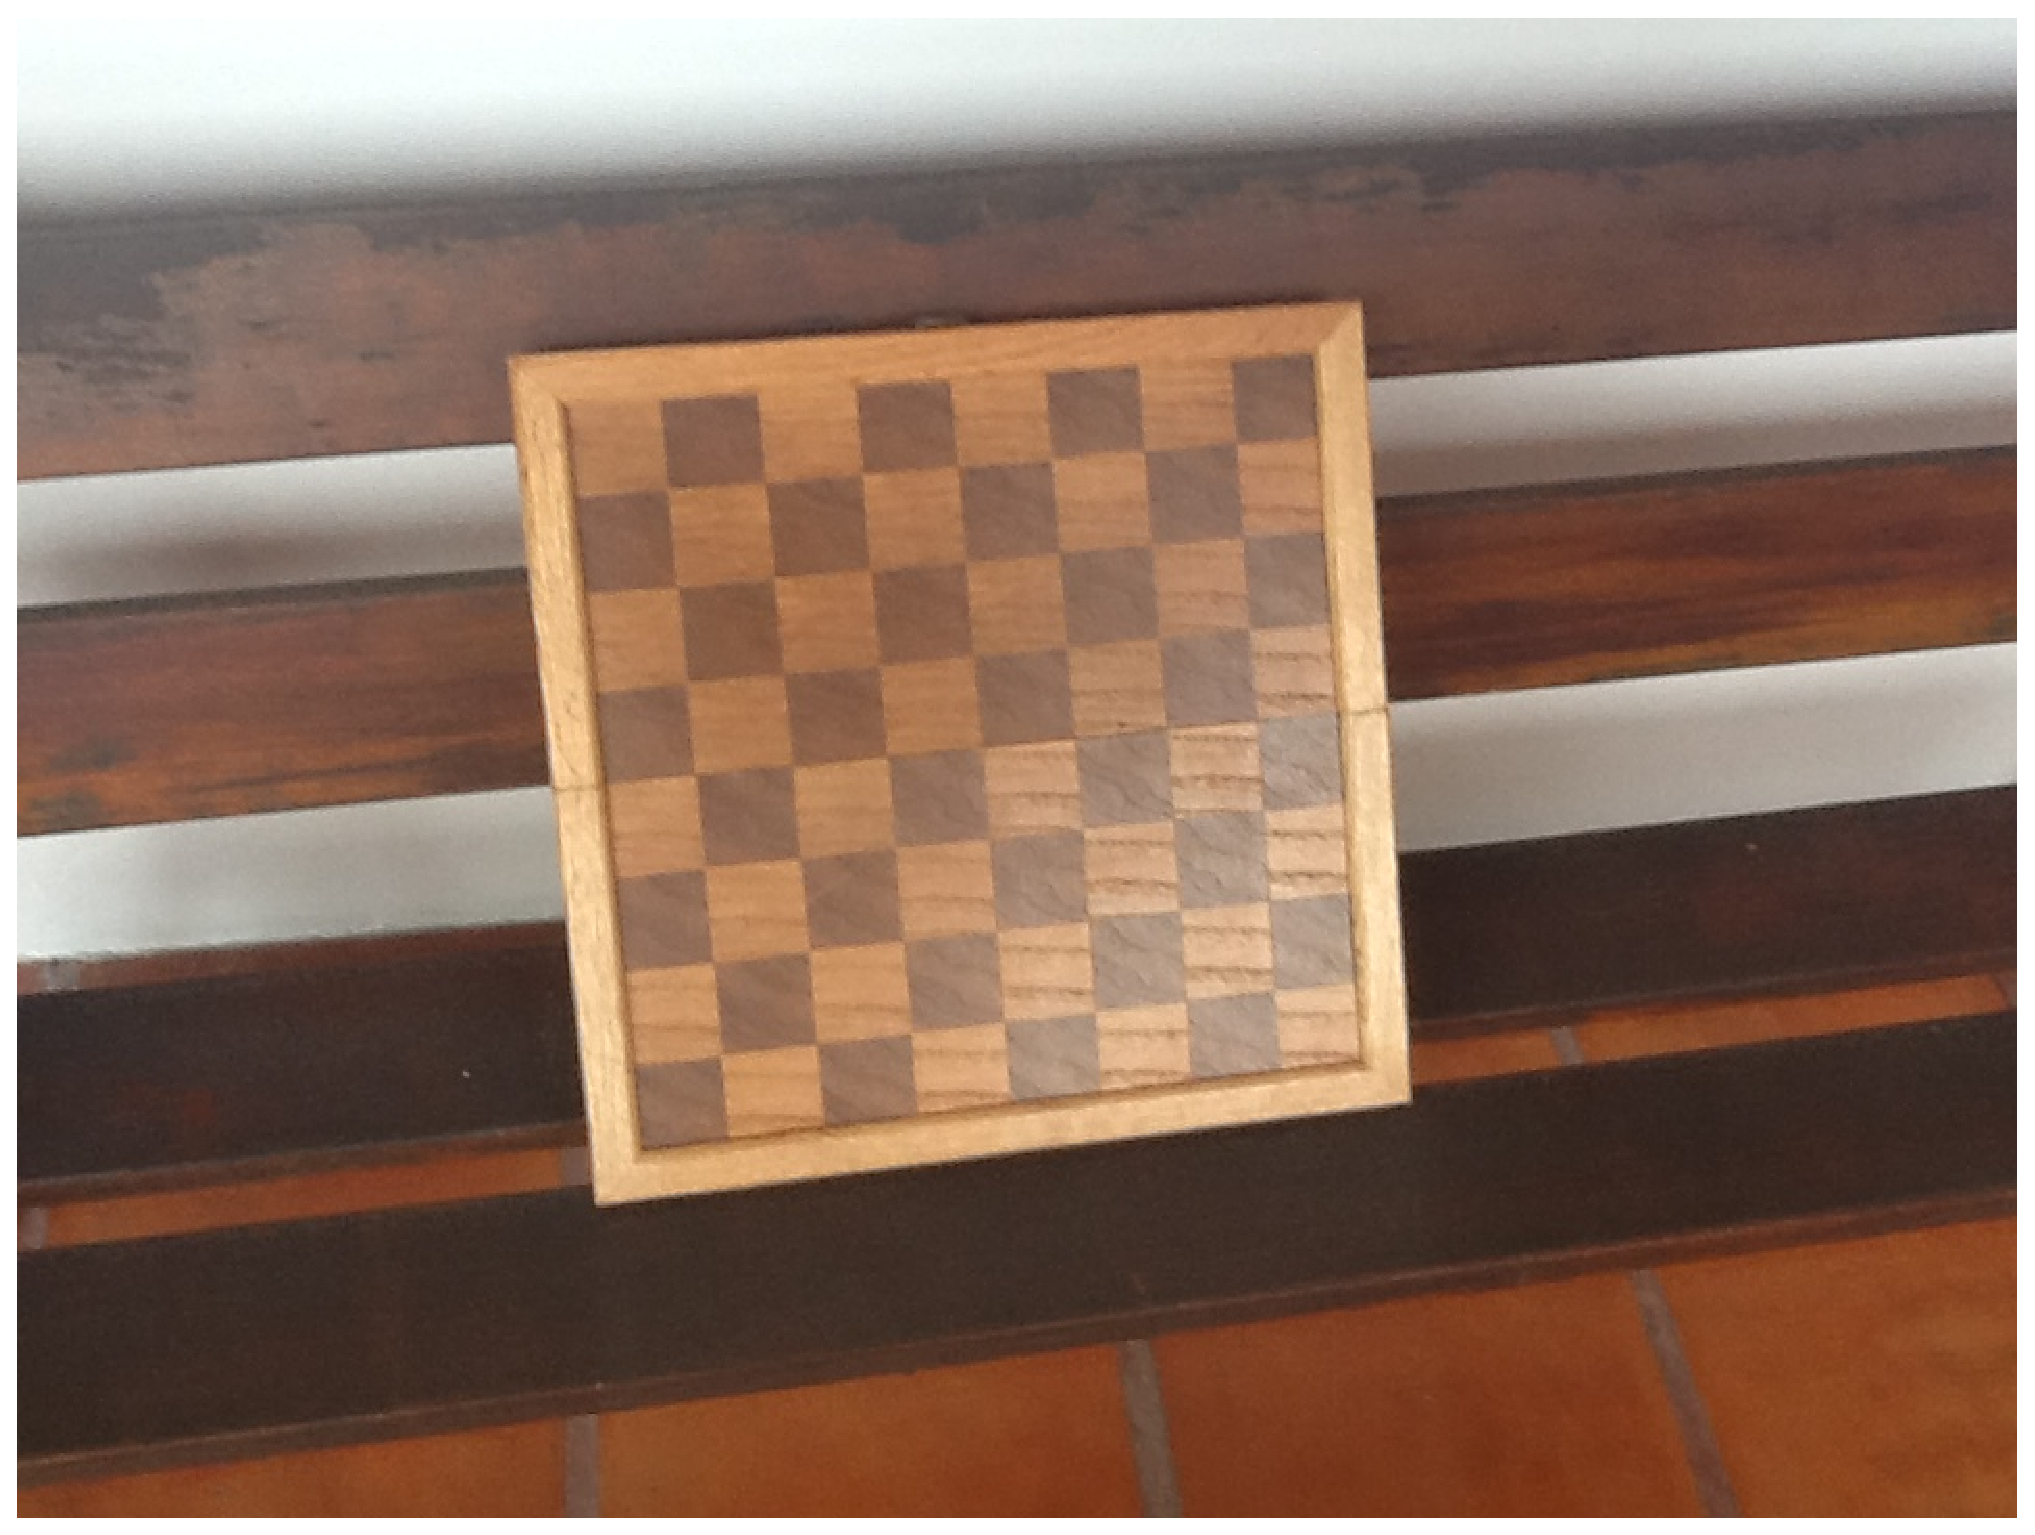
\includegraphics[scale=0.2]{figs_camaraypose/damero}
\caption{Imagen de un damero, utilizada para calibrar la c�mara del \textit{iPad} durante el proyecto.}
\label{fig:damero}
\end{figure}

El m�todo de Zhang es muy sencillo y flexible. S�lo requiere de la c�mara a calibrar, una computadora y una imagen patr�n (plana), de tipo damero; a la que se le tomar�n al menos dos fotograf�as desde orientaciones distintas. En la figura \ref{fig:damero} se ve una de las im�genes utilizadas para calibrar la c�mara del \textit{iPad} durante el proyecto. Ni las posiciones de la c�mara en cada caso, ni el movimiento entre estas posiciones tienen por qu� ser conocidos. Este m�todo devuelve los par�metros intr�nsecos de la c�mara correspondientes al modelo \textit{pin-hole} visto anteriormente, sus par�metros extr�nsecos para cada fotograf�a utilizada para la calibraci�n y la distorsi�n radial de sus lentes.\\

Recu�rdese que la relaci�n entre un punto 3D \textbf{M} expresado respecto de los ejes de coordenadas del mundo y su proyecci�n en el plano imagen \textbf{m}, expresada respecto de los ejes normalizados de la imagen, viene dada por:
\[
m = I.E.M
\]
donde $E$ representa a la matriz de par�metros extr�nsecos e $I$ representa a la matriz de par\'ametros intr�nsecos de la c�mara. Adem�s:
\[
I =
\left( \begin{array}{ccc}
\alpha & s & x'_C\\ 
0 & \beta & y'_C\\
0 & 0 & 1
\end{array} 
\right)
\]
con $\alpha = d_x.f$ y $\beta = d_y.f$.\\ 

Se asume en este m�todo que el sistema de coordenadas del mundo ``reposa'' sobre la imagen patr�n; o lo que es lo mismo, que esta se encuentra en $Z=0$. Se obtiene entonces la siguiente simplificaci�n:\\
\[
\left( \begin{array}{c}
x'_0 \\
y'_0 \\
1
\end{array} \right)
= 
I
.
\left( \begin{array}{cccc}
r_{1} & r_{2} & r_{3} & t
\end{array} \right)
.
\left( \begin{array}{c}
U_0 \\ 
V_0 \\
W_0 \\
1
\end{array} \right)
=
I
.
\left( \begin{array}{cccc}
r_{1} & r_{2}  & t
\end{array} \right)
.
\left( \begin{array}{c}
U_0 \\ 
V_0 \\
1
\end{array} \right)
\]
donde $(U_0, V_0,W_0, 1 )^T$ denota las coordenadas homog�neas del punto \textbf{M} respecto de los ejes del mundo y $(x'_0,y'_0,1)^T$ representa las coordenadas homog�neas de su proyecci�n en el plano imagen, \textbf{m}, respecto de los ejes normalizados de la imagen. Se le llam� $r_i$ a la i-�sima columna de la matriz rotaci�n de los par�metros extr�nsecos de la c�mara.\\

Dada una fotograf�a de la imagen patr�n plana (figura \ref{fig:damero}), es posible estimar una homograf�a que relacione a los puntos de la imagen con sus correspondientes en la fotograf�a. Si se toma en cuenta que dicha homograf�a vale $H =(h_{1}, h_{2}, h_{3}) = I.(r_{1}, r_{2}, t)$, con $h_i$ la i-�sima columna de la matriz, y que las columnas $r_1$ y $r_2$ son ortonormales entre s�, realizando algo de matem�tica se llega a que:
\[
\begin{array}{c}
h_1^T.(I^{-1})^T.I^{-1}.h_2 =0 \\
h_1^T.(I^{-1})^T.I^{-1}.h_1 =h_2^T.(I^{-1})^T.I^{-1}.h_2 \\
\end{array}
\]
Las anteriores son las �nicas dos relaciones b�sicas entre par�metros intr�nsecos que se pueden obtener a partir de una �nica homograf�a. Esto es porque una homograf�a tiene 8 grados de libartad y existen 6 par�metros extr�nsecos (3 para la traslaci�n y 3 para la rotaci�n).\\

Si se define la matriz $B$ como sigue:
\[
B = (I^{-1})^T.I^{-1} = 
\left( \begin{array}{ccc}
B_{11} & B_{21} & B_{31}\\ 
B_{12} & B_{22} & B_{32}\\
B_{13} & B_{23} & B_{33}
\end{array} 
\right)
=
\left( \begin{array}{ccc}
\frac{1}{\alpha^2} 										& -\frac{s}{\alpha^2.\beta} 																			& \frac{s.v_P' - u_P'.\beta}{\alpha^2.\beta} \\
 -\frac{s}{\alpha^2.\beta}  							&  \frac{s^2}{\alpha^2.\beta^2} + \frac{1}{\beta^2} 									& -\frac{s(s.v_P' - u_P'.\beta)}{\alpha^2.\beta^2} - \frac{v_P'}{\beta^2} \\
\frac{s.v_P' - u_P'.\beta}{\alpha^2.\beta}	& -\frac{s(s.v_P' - u_P'.\beta)}{\alpha^2.\beta^2} - \frac{v_P'}{\beta^2}		& \frac{(s.v_P' - u_P'.\beta)^2}{\alpha^2.\beta^2} + \frac{v_P'^2}{\beta^2} +1
\end{array} \right)
\]
se ve f�cilmente que esta es sim�trica, por lo que quedar� absolutamente definida por un vector de 6 dimensiones:
\[
b = (B{11}, B_{12}, B_{22}, B_{13}, B_{23}, B_{33})^T
\]
Si adem�s se define el vector variable $v_{ij}$ de la siguiente manera:
\[
v_{ij} = (h_{i1}.h_{j1}, h_{i1}.h_{j2}+h_{i2}.h_{j1}, h_{i2}.h_{j2},  h_{i3}.h_{j1}+h_{i1}.h_{j3}, h_{i3}.h_{j2}+h_{i2}.h_{j3}, h_{i3}.h_{j3})^T,
\]
se tiene que:
\[
h_i^T.B.h_j = V_{ij}^T.b
\]
Las dos relaciones b�sicas entre par�metros intr�nsecos obtenidas de una �nica homograf�a, vistas anteriormente, pueden ser reescritas como:
\[
\left(
\begin{array}{c}
v_{12}^T \\
(v_{11} - v_{22})^T
\end{array}
\right)
.b = V.b = 0
\]
Utilizando $n$ fotograf�as distintas de la imagen patr�n, y por lo tanto $n$ homograf�as distintas se obtiene una matriz V de tama\~no $2.n\times 6$. Es sabido que si $n\geq 3$, el sistema matricial anterior tendr� una soluci�n $b$ �nica, que var�a seg�n cierto factor de escala. Sin embargo, si $n=2$, es posible imponer la condici�n $s=0$ y as� tambi�n calcular al vector $b$ de forma �nica, sin mayores problemas.\\

Una vez estimado $b$ es posible recontruir la matriz de par�metros intr�nsecos I, para luego utilizando I y las homograf�as H obtener los par�metros extr�nsecos de la c�mara para cada fotograf�a utilizada para la calibraci�n.\\ 

El art�culo de Zhang afirma que la soluci�n obtenida hasta el momento no es del todo buena, pues se obtuvo minimizando una distancia algebraica y eso no tiene mucho sentido. Lo que se hace entonces es, utilizando las $n$ fotograf�as tomadas para la calibraci�n y los $k$ puntos seleccionados en cada una de ellas, minimizar la siguiente ecuaci�n:
\[
\sum_{i=1}^{n} \sum_{j=1}^{k}  \norm{m_{ij} - \hat{m}(I, E_i, M_j)}^2
\]
donde $\hat{m}(I, E_i, M_j)$ es la proyecci�n del punto $M_j$ en la imagen $i$ utilizando la homograf�au $H_i= I.E_i$. El resultado de dicha minimizaci�n no lineal ser� el resultado final. Este m�todo requiere de valores inicales para $I$ y para los $E_i|_{i=1..n}$; que ser�n los obtenidos en los c�lculos anteriores. \\

Finalmente se realiza una estimaci�n de la distorsi�n radial utilizando un modelo muy similar al visto en la secci�n \ref{sec:distorsion}. Cabe destacar que cuando se estimaron los par�metros intr�nsecos de las c�maras utilizadas en este proyecto, la distorsi�n radial no se tom� en cuenta y a�n as� los resultados obtenidos fueron realmente muy precisos.\\

\section{Problema de estimaci�n de pose}\label{sec:Problema de estimaci�n de pose}
Como se mencion� en \ref{sec:Fundamentos y definiciones} la matriz de par�metros extr�nsecos \textit{E} representa a la pose de la c�mara. El problema de estimaci�n de pose consiste en determinar esta matriz dadas $n$ correspondencias entre puntos $M_i$ en el mundo 3D y puntos $m_i$ en la imagen. 

Existen varios algoritmos de estimaci�n de pose, a continuaci�n se presentan algunos. 

\subsection{\textit{DLT}(\textit{D}irect \textit{L}inear \textit{T}ransform)}
Este m�todo sirve para calcular la matriz \textbf{H} en la cual est�n impl�citos los par�metros intr�nsecos y extr�nsecos. Si se conocen los par�metros intr�nsecos se pueden despejar la matriz \textbf{E} con la informaci�n de la pose. 

Como se vio anteriormente

\[
\left( \begin{array}{c}
x_i \\
y_i \\
s_i
\end{array} \right)
= 
\left( \begin{array}{cccc}
\textbf{H}_{11} & \textbf{H}_{12} & \textbf{H}_{13} & \textbf{H}_{14} \\ 
\textbf{H}_{21} & \textbf{H}_{22} & \textbf{H}_{23} & \textbf{H}_{24}\\
\textbf{H}_{31} & \textbf{H}_{32} & \textbf{H}_{33} & \textbf{H}_{34} \\
\textbf{H}_{41} & \textbf{H}_{42} & \textbf{H}_{43} & \textbf{H}_{44}
\end{array} \right)
.
\left( \begin{array}{c}
U_i \\ 
V_i \\
W_i \\
P_i
\end{array} \right)
\] 

Por comodidad a partir de ahora cuando se refiera a puntos 2D $(x_i,y_i)$ ser�n expresados siempre desde el eje de coordenadas normalizadas de la imagen. Se debe notar que la matriz \textbf{H}  puede ser multiplicada por un factor distinto de cero sin alterar el resultado de la proyecci�n, esto se debe a que se trabaja con coordenadas homog�neas. Por lo tanto lo que define la proyecci�n no son los elementos de \textbf{H} sino la relaci�n entre todos los elementos (excepto el de factor de escala) y el elemento que da el factor de escala. As� entonces \textbf{H} tiene 12 elementos pero solamente 11 grados de libertad.
 
Cada correspondencia $M_i \leftrightarrow m_i$ aporta dos ecuaciones linealmente independientes con los elementos de la matriz \textbf{H}, $\textbf{H}_{ij}$ como variables
\begin{equation*}
\begin{split}
\frac{\textbf{H}_{11}X_i+\textbf{H}_{12}Y_i+\textbf{H}_{13}Z_i+\textbf{H}_{14}}{\textbf{H}_{31}X_i+\textbf{H}_{32}Y_i+\textbf{H}_{33}Z_i+\textbf{H}_{34}} = x_i, \\
\\
\frac{\textbf{H}_{21}X_i+\textbf{H}_{22}Y_i+\textbf{H}_{23}Z_i+\textbf{H}_{24}}{\textbf{H}_{31}X_i+\textbf{H}_{32}Y_i+\textbf{H}_{33}Z_i+\textbf{H}_{34}} = y_i 
\end{split}
\end{equation*}
La ecuaci�n para $s_i$ se puede obtener como combinaci�n lineal de las de $x_i$ y $y _i$, por eso no se tiene en cuenta. 
Estas ecuaciones se pueden reescribir como $\textbf{A}h=0$ donde 
\begin{equation*}
h = \left(
\begin{array}{cccccccccccc}
\textbf{H}_{11} & \textbf{H}_{12} & \textbf{H}_{13} & \textbf{H}_{14} & \textbf{H}_{21} & \textbf{H}_{22} & \textbf{H}_{23} & \textbf{H}_{24} & \textbf{H}_{31} & \textbf{H}_{32} & \textbf{H}_{33} & \textbf{H}_{34} 
\end{array}
\right)^T
\end{equation*}
y 
\begin{equation*}
\textbf{A} = \footnotesize
\left(
\begin{array}{cccccccccccc}
X_0 & Y_0 & Z_0 & 1 & 0 & 0 & 0 & 0 & -x_0X_0 & -x_0Y_0 & -x_0Z_0 & -x_0\\
0 & 0 & 0 & 0 & X_0 & Y_0 & Z_0 & 1 & -y_0X_0 & -y_0Y_0 & -y_0Z_0 & -y_0 \\
X_1 & Y_1 & Z_1 & 1 & 0 & 0 & 0 & 0 & -x_1X_1 & -x_1Y_1 & -x_1Z_1 & -x_1\\
0 & 0 & 0 & 0 & X_1 & Y_1 & Z_1 & 1 & -y_1X_1 & -y_1Y_1 & -y_1Z_1 & -y_1 \\
\vdots & \vdots & \vdots & \vdots &\vdots & \vdots &\vdots & \vdots & \vdots & \vdots & \vdots & \vdots\\
X_{n-1} & Y_{n-1} & Z_{n-1} & 1 & 0 & 0 & 0 & 0 & -x_{n-1}X_{n-1} & -x_{n-1}Y_{n-1} & -x_{n-1}Z_{n-1} & -x_{n-1}\\
0 & 0 & 0 & 0 & X_{n-1} & Y_{n-1} & Z_{n-1} & 1 & -y_{n-1}X_{n-1} & -y_{n-1}Y_{n-1} & -y_{n-1}Z_{n-1} & -y_{n-1} \\
\end{array}
\right)
\normalsize
\end{equation*}
La transformaci�n obtenida la matriz \textbf{H} tiene 11 grados de libertad como mencion� anteriormente, por lo tanto el rango de la matriz \textbf{A} es 11. Se realiza la descomposici�n SVD de la matriz \textbf{A}, el vector propio del valor singular de \textbf{A} con valor menor es la base del n�cleo de \textbf{A}. Entonces se tiene que $h$ es este vector a menos de una constante.  Una vez que se tiene $h$ se puede armar la matriz \textbf{H}. Luego se tiene que 
$$\textbf{E} = \textbf{I}^{-1}\textbf{H}$$

\subsection{\textit{PnP} (\textit{P}erspective-\textit{n}-\textit{P}oint)}
Si se cuenta con los par�metros intr�nsecos, se puede utilizar un enfoque que se centre en calcular solamente la pose de la c�mara. Dependiendo de la cantidad de correspondencias que se tienen entre la imagen y el modelo es posible obtener un n�mero finito de soluciones de la pose. 
Si se tienen 1 o 2 correspondencias el problema tiene infinitas soluciones. Si se tienen 3 correspondencias(P3P) se obtienen hasta 4 posibles soluciones. Para 4 o m�s correspondencias se obtiene una �nica soluci�n, siempre que los puntos no est�n alineados.
La idea detr�s de este algoritmo es la siguiente: 
\begin{itemize}
\item[$\bullet$] A partir de los puntos de la imagen $m_i$ y conociendo la distancia focal $f$ es posible calcular los versores $j_i$. 
$$ j_i = \frac{1}{\sqrt{x_i^2 + y_i^2 + f^2}}\left(\begin{array}{c}
x_i \\
y_ i\\
f
\end{array}\right)
$$
\item[$\bullet$] Con estos versores es posible determinar los �ngulos que forman las lineas de vista de los puntos $\textbf{M}_i$ entre s�. 
\item[$\bullet$] Se busca estimar las distancias $l_i = \Vert\textbf{O}\textbf{M}_i\Vert$ entre el centro de la c�mara y los puntos 3D $\textbf{M}_i$ a partir de las relaciones dadas por los tri�ngulos $\textbf{O}\textbf{M}_i\textbf{M}_j$.
\item[$\bullet$]  Una vez que se calculan las distancias $l_i$, los puntos $\textbf{M}_i$ se expresan en el sistema de coordenadas de la c�mara como $\textbf{M}^\textbf{C}_i$. 
\item[$\bullet$] Finalmente \textbf{R} y \textbf{T} quedan determinadas como la transformaci�n que lleva puntos en el sistema de coordenadas del mundo a el sistema de coordenadas de la c�mara.
\end{itemize}
En la bibliograf�a \cite{Fischler} y \cite{Haralick} se encuentran varios m�todos para resolver num�ricamente el problema. 
\begin{figure}[h]
\centering
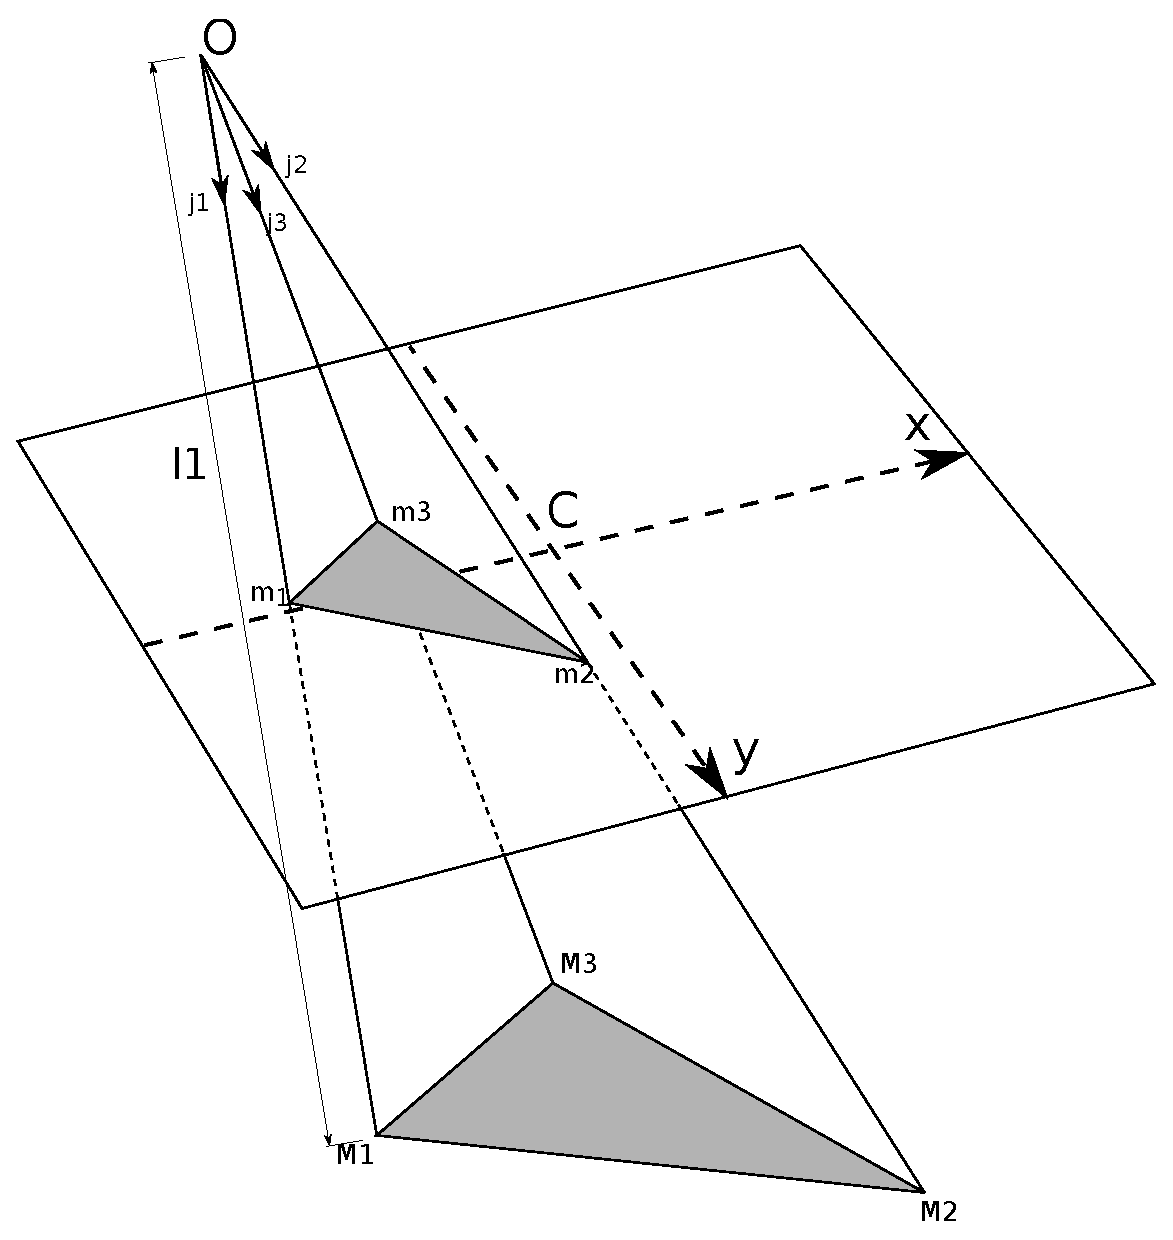
\includegraphics[scale=0.55]{figs_camaraypose/pnp}
\caption{Geometr�a del problema P3P. Se busca calcular la distancia entre el centro �ptico $O$ y los puntos del modelo 3D}
\label{fig:pnp}
\end{figure}


\subsection{RANSAC(RANdom SAmple Consensus)}
Este es un algoritmo iterativo utilizado para estimar los par�metros de un modelo matem�tico de un conjunto de datos que contiene \textit{outliers} (datos fuera del modelo). En particular se puede utilizar para el problema de estimaci�n de pose cuando no se tienen las correspondencias entre puntos detectados y puntos del modelo. 

A continuaci�n se presenta el algoritmo:
\begin{itemize}
\item[(1)] Dado un modelo que requiere un m�nimo de \textit{n} puntos para determinar sus par�metros, y un conjunto de datos \textbf{P} tal que el n�mero de puntos en \textbf{P} es mayor que \textit{n}, se sortea un subconjunto $S_1$ de \textit{n} puntos de \textbf{P} para instanciar el modelo. Con el modelo instanciado $\textbf{M}_1$ se determina el subconjunto de decisi�n $S_1^*$ de puntos de \textbf{P} que est�n a menos de una distancia \textit{t} de $\textbf{M}_1$.

\item[(2)] Si la cantidad de puntos en $S_1^*$  es mayor que un umbral \textbf{T} entonces se elige el subconjunto de decisi�n $S_1^*$ para computar el nuevo modelo $\textbf{M}_1^*$.

\item[(3)] Si la cantidad de puntos en $S_1^*$ es menor que \textbf{T}, se sortea un nuevo subconjunto $S_2$ y se repite el proceso. Si luego de una cantidad de \textit{N} n�mero de pruebas no se obtiene un subconjunto de decisi�n que cumple con el umbral \textbf{T}, se resuelve el modelo con el subconjunto de decisi�n mas grande obtenido, o se termina sin devolver modelo.
\end{itemize}
Los par�metros \textit{t}, \textbf{T} y \textit{N}, se eligen en base al modelo a estimar y a la probabilidad de encontrar un \textit{outlier} en el conjunto de datos . 


 \subsection{POSIT}
Este es un algoritmo iterativo que se basa en utilizar la proyecci�n ortogonal escalada (SOP) para resolver el problema de estimaci�n de pose. Se necesita tener m�s de cuatro correspondencias entre puntos del modelo $M_i$ y puntos en la imagen $m_i$. De todos los algoritmos presentados este fue el que se decidi� utilizar. El desarrollo de la teor�a de este algoritmo se encuentra en \ref{ch: posit}. 
Este algoritmo tiene diferentes variantes. Por un lado esta la versi�n original del algoritmo y una versi�n que resuelve el caso en que todos los puntos del modelo est�n en un mismo plano, (POSIT Coplanar). Luego se tiene una variante llamada SoftPOSIT que resuelve la estimaci�n de pose sin la necesidad de conocer las correspondencias entre puntos del modelo 3D y puntos de la imagen en el caso en que los puntos del modelo no sean coplanares. Finalmente se tiene una variante de SoftPOSIT que trabaja con l�neas.

La variante de SoftPOSIT de l�neas fue el principal argumento para tomar la decisi�n ya que el detector de caracter�sticas que se usa es el LSD\ ref{ch: lsd}. Esta variante fue implementada sin �xito, pero en busca de esta implementaci�n se desarroll� una versi�n de POSIT para puntos coplanares que no est� presentada en la bibliograf�a y dio buenos resultados. Otro argumento a favor de esta opci�n es que se contaba con implemetaciones de algunas variantes. De \cite{DeMenthonCoplanarCode} se obtuvieron las implementaciones de POSIT y POSIT coplanar en C y la implementaci�n en MatLab de SoftPOSIT. Para la variante de SoftPOSIT de l�neas s�lo se cont� con el art�culo\cite{SoftLine}.

\section{Representaci�n de la pose de la c�mara}\label{sec:Representaci�n de la pose de la c�mara}
Como se vio anteriormente, la pose de la c�mara queda determinada por una matriz de rotaci�n \textbf{R} y un vector de traslaci�n \textbf{T}. La matriz \textbf{R} indica la orientaci�n de la c�mara respecto al mundo. Hay varias maneras de representar esta orientaci�n, entre ellas se encuentran la representaci�n matricial, la representaci�n en �ngulos de Euler y los \textit{quaternions}. Dependiendo de la aplicaci�n puede resultar m�s �til utilizar las diferentes representaciones. 

\subsection{Representaci�n matricial}
Esta representaci�n es la que se introdujo en \ref{sec:Matriz de proyecci�n}. En esta matriz las filas corresponden a los versores del sistema de coordenadas de la c�mara expresados en las coordenadas del mundo. Se puede expresar como
\[
\textbf{R} = \left(\begin{array}{ccc}
i_u & i_v & i_w \\
j_u & j_v & j_w  \\
k_u & k_v & k_w 
\end{array}\right)
\]
La ventaja que tiene esta representaci�n es que el pasaje de puntos en coordenadas del mundo a coordenadas de la c�mara es directo, simplemente se multiplica por la matriz \textbf{R} al punto en coordenadas del mundo y se le suma el vector de traslaci�n. 

\subsection{�ngulos de Euler}
La matriz de rotaci�n \textbf{R} se puede escribir como un producto de matrices que representan las rotaciones alrededor de los ejes $x$, $y$ y $z$. No hay ninguna convenci�n establecida en cuanto al orden en que se realizan las rotaciones. Por ejemplo si se toman $\psi$, $\theta$ y $\phi$ como los �ngulos de rotaci�n en torno a $x$, $y$ y $z$ respectivamente se tiene 
\[
\textbf{R}=R_z(\phi)R_y(\theta)R_x(\psi)=\left(\begin{array}{ccc}
\cos \phi & -\sin \phi & 0 \\
\sin \phi & \cos \phi & 0 \\
0 & 0 & 1
\end{array}\right)  
\left(\begin{array}{ccc}
\cos \theta & 0 & \sin \theta \\
0 & 1 & 0\\
-\sin \theta & 0 & \cos \theta
\end{array}\right)  
\left(\begin{array}{ccc}
1 & 0 & 0 \\
0 & \cos \psi & -\sin \psi \\
0 & \sin \psi & \cos \psi \\
\end{array}\right)  
\]

Desarrollando el producto se tiene que 
\[
\textbf{R} = \left(\begin{array}{ccc}
\cos \theta \cos \phi & \sin\psi\sin\theta\cos\phi - \cos\psi\cos\phi & \cos\psi\sin\theta\cos\phi + \sin\psi\sin\phi \\
 \cos\theta\sin\phi & \sin\psi\sin\theta\sin\phi+\cos\psi\cos\phi & \cos\psi\sin\theta\sin\phi-\sin\psi\cos\phi \\
-\sin\theta & \sin\psi\cos\theta & \cos\psi\cos\theta
\end{array}\right)
\]

\subsubsection{Orden de rotaciones}
Cuando se trabaja con matrices de rotaciones y �ngulos de Euler es necesario saber en qu� orden se aplican las rotaciones, pues no es una transformaci�n conmutativa. Un objeto rotado primero seg�n el eje $x$ y luego seg�n el eje $y$ termina en una posici�n diferente que si se lo rota primero seg�n $y$ y luego seg�n $x$. Esto se puede ver en la Figura \ref{fig: mono3}.

\begin{figure}[h!]\label{fig: mono3}
\centering
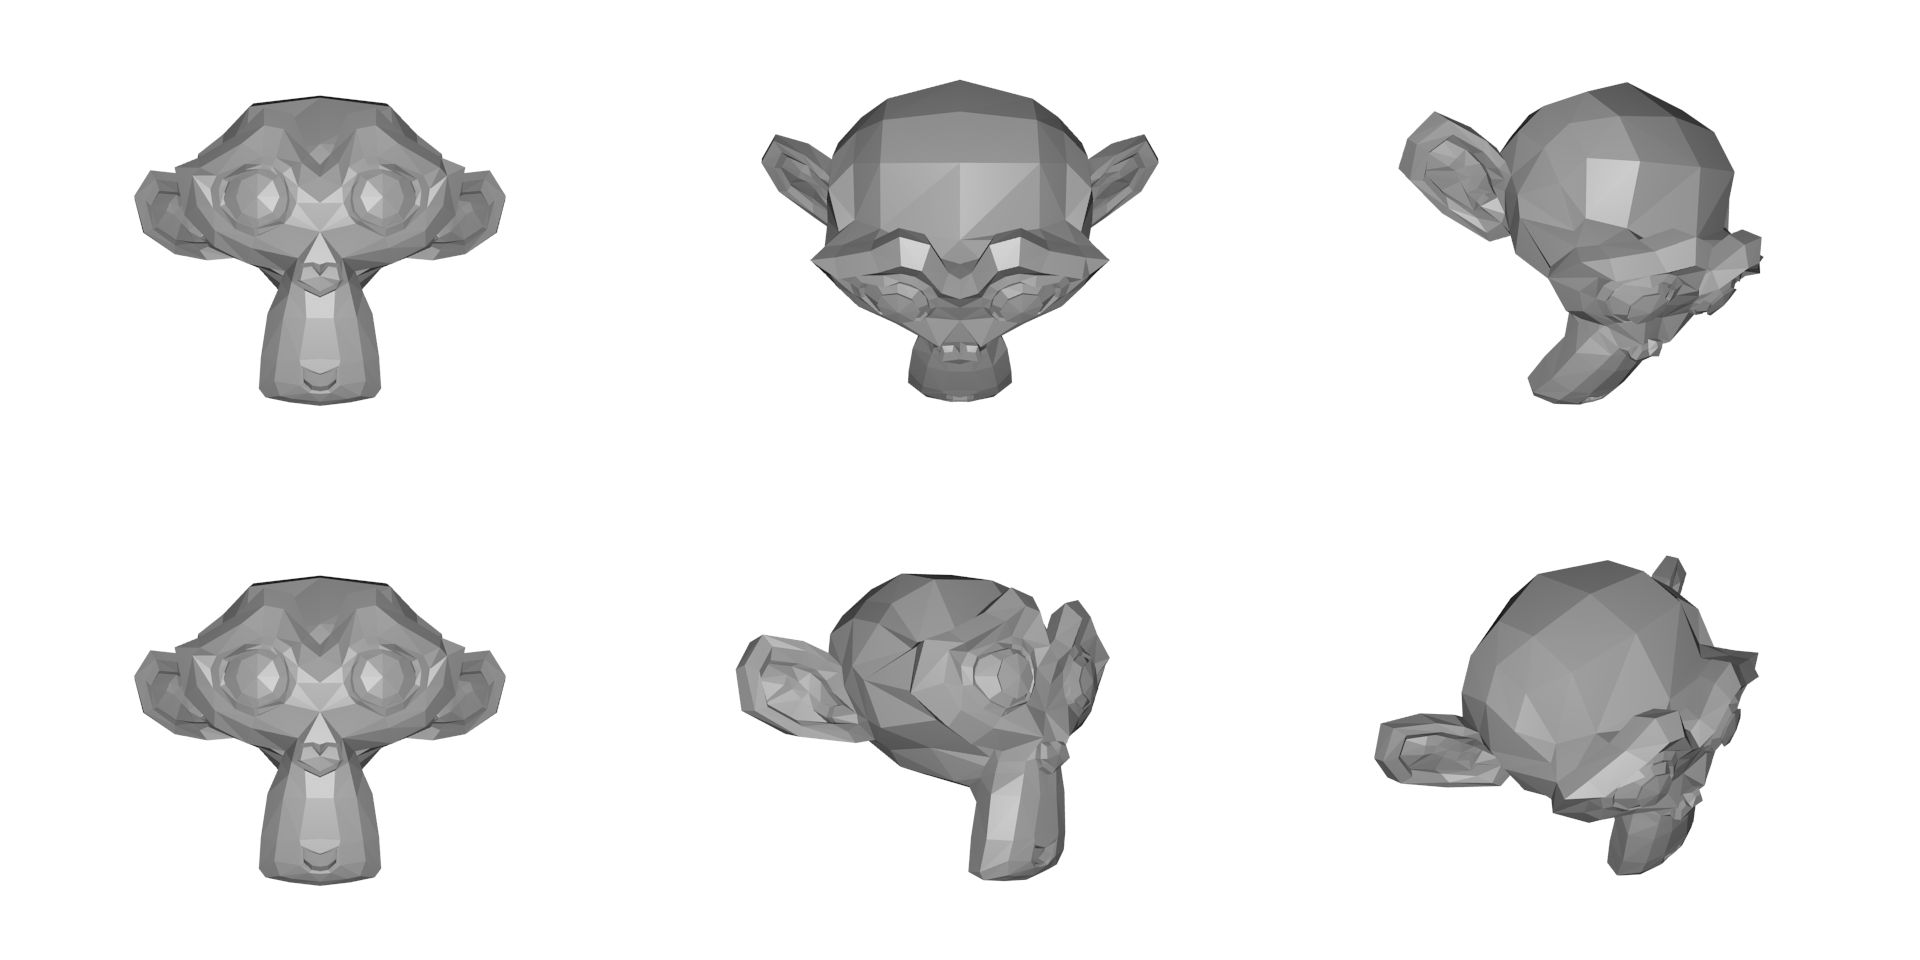
\includegraphics[scale=0.5]{figs_camaraypose/mono3}
\caption{Se parte del mismo objeto, en la fila superior se aplica una rotaci�n de $45^\circ$ seg�n $x$ y luego una rotaci�n de $45^\circ$ seg�n $y$. En la fila de abajo se aplican las mismas rotaciones pero en orden inverso. Se puede ver que se obtienen diferentes posiciones.}
\label{fig:mono3}
\end{figure}



\subsubsection{C�lculo de los �ngulos de Euler}
Si se tiene la matriz \textbf{R} es posible realizar la descomposici�n y obtener los �ngulos de Euler. De $\textbf{R}_{31}$ se obtiene el valor de $\theta$
$$ \theta = -\arcsin(\textbf{R}_{31}).$$
Como $\sin(\theta)=\sin(\pi -\theta)$, puede haber dos posibles valores de $\theta$(si $\textbf{R}_{31}\neq \pm 1$)
\begin{equation}\label{eq_1}
\begin{split}
\theta_1 &= -\arcsin(\textbf{R}_{31}) \\
\theta_2 &= \pi - \theta_1 = \pi + \arcsin(\textbf{R}_{31})
\end{split}
\end{equation}

 A partir de estos valores de $theta$ es posible encontrar dos juegos de �ngulos que dan la misma matriz \textbf{R}. Para calcular $\psi$ se observa que 
 \[
 \frac{\textbf{R}_{32}}{\textbf{R}_{33}} = \tan\psi
\]
 de donde se deduce que 
 \[
 \psi = \arctan \left( \frac{\textbf{R}_{32}}{\textbf{R}_{33}}\right)
 \]
 Es importante obtener el cuadrante al que pertenece el �ngulo, por esto es que se usa la funci�n $\arctan2$ que esta disponible en $C$, recordar que la imagen de $\arctan$ es $[-\pi /2, \pi /2]$ por lo que hay 2 cuadrantes que no se consideran. Como en los t�rminos $\textbf{R}_{32}$ y $\textbf{R}_{33}$ aparece el t�rmino $\cos\theta$ multiplicando, hay que tener en cuenta su signo para obtener el valor de $\psi$. Si $\cos(\theta)>0$, se tiene que $\psi = \arctan\left(\textbf{R}_{32} / \textbf{R}_{33}\right)$. Si $\cos(\theta)<0$, $\psi = \arctan\left(-\textbf{R}_{32} / -\textbf{R}_{33}\right)$. Para tener en cuenta esto se toma
 \[
 \psi = \arctan\left(\frac{\textbf{R}_{32} / \cos\theta}{\textbf{R}_{33} / \cos\theta}\right)
 \]
  Por lo tanto los dos posibles valores para $\psi$ son
\begin{equation}\label{eq_2}
\begin{split}
 \psi_1 &= \arctan\left(\frac{\textbf{R}_{32}/\cos\theta_1}{\textbf{R}_{33}/\cos\theta_1}\right)\\
 \psi_2 &= \arctan\left(\frac{\textbf{R}_{32}/\cos\theta_2}{\textbf{R}_{33}/\cos\theta_2}\right)
\end{split} 
 \end{equation}

  De manera similar se puede obtener $\phi$. Se observa que
  \[
  \frac{\textbf{R}_{21}}{\textbf{R}_{11}} = \tan\phi
  \]
  por lo tanto se llega a
\begin{equation}\label{eq_3}
\begin{split}
 \phi_1 &= \arctan\left(\frac{\textbf{R}_{21}/\cos\theta_1}{\textbf{R}_{11}/\cos\theta_1}\right)\\
 \phi_2 &= \arctan\left(\frac{\textbf{R}_{21}/\cos\theta_2}{\textbf{R}_{11}/\cos\theta_2}\right)
\end{split}
\end{equation}
Las ecuaciones \ref{eq_2} y \ref{eq_3} son v�lidas para el caso en que $\cos\theta \neq 0$

En el caso en que $\cos\theta = 0$ se tiene que $\theta = \pm \pi/2$, ademas los t�rminos $\textbf{R}_{11}$, $\textbf{R}_{21}$, $\textbf{R}_{32}$ y $\textbf{R}_{33}$ son nulos. Por lo tanto se utilizan otros elementos de la matriz de rotaci�n para hallar los �ngulos restantes. 
En el caso en que  $\theta = \pi/2$ se tiene que 
\begin{equation*}
\begin{split}
\textbf{R}_{12} &=  \sin\psi\cos\phi - \cos\psi\cos\phi = \sin\left(\psi - \phi\right) \\
\textbf{R}_{13} &=  \cos\psi\cos\phi + \sin\psi\sin\phi = \cos\left(\psi - \phi\right) \\
\textbf{R}_{22} &=  \sin\psi\sin\phi + \cos\psi\cos\phi = \cos\left(\psi - \phi\right) = \textbf{R}_{13}\\
\textbf{R}_{23} &=  \cos\psi\sin\phi - \sin\psi\cos\phi = -\sin\left(\psi - \phi\right)  = -\textbf{R}_{12}
\end{split}
\end{equation*}
Cualquier $\psi$ y $\phi$ que verifiquen estas ecuaciones ser�n soluciones v�lidas. Usando las ecuaciones para $\textbf{R}_{12}$ y $\textbf{R}_{13}$ se tiene que
\begin{align*}
\centering
\left(\psi - \phi\right) =&  \arctan\left(\textbf{R}_{12}/\textbf{R}_{13}\right) \\
\psi =&  \phi + \arctan\left(\textbf{R}_{12}/\textbf{R}_{13}\right) \\
\end{align*}
Para el caso en que $\theta = -\pi/2$ se procede de igual manera y se llega a que 
\begin{align*}
\centering
\left(\psi + \phi\right) =&  \arctan\left(-\textbf{R}_{12}/-\textbf{R}_{13}\right) \\
\psi =&  - \phi + \arctan\left(-\textbf{R}_{12}/-\textbf{R}_{13}\right) \\
\end{align*}

\subsubsection{Gimbal lock}
La gran desventaja que presenta la representaci�n de la rotaci�n mediante �ngulos de Euler, es el problema denominado \textit{gimbal lock}. Este problema se da cuando 2 de los ejes de rotaci�n quedan alineados. Si hay dos ejes alineados, se pierde un grado de libertad ya que los dos ejes rotan de la misma manera. Para la composici�n de rotaciones que se utilizan en la aplicaci�n el \textit{gimbal lock} se da cuando se gira $\pi/2$ seg�n $y$. Como se vio anteriormente, en el caso en que $\theta = \pi/2$ la matriz de rotaci�n queda
\[
\textbf{R} = \left(\begin{array}{ccc}
0 & \sin\left(\psi - \phi\right)  & \cos\left(\psi - \phi\right)\\
0 & \cos\left(\psi - \phi\right) & -\sin\left(\psi - \phi\right) \\
-1 & 0 & 0
\end{array}\right)
\]
Esto es una rotaci�n entorno al vector $(0,0,-1)$ de un �ngulo $\alpha=\psi-\phi$

Esto se puede ver gr�ficamente en la Figura \ref{fig: gimbal}. Se realiza la rotaci�n seg�n $y$ y se pueden ver que los ejes de $x$ y $z$ quedan alineados. Luego se realiza una rotaci�n de $60^\circ$ en torno a $x$ y por otra parte tambi�n se hace otra igual pero de signo opuesto en torno a $z$. Se ve que la posici�n final, partiendo de los ejes alineados para una y otra rotacio�n del modelo es la misma. Lo que cambia es la posici�n del eje $y$. Cuando se rota en torno a $x$, el eje $y$ queda quieto porque est� m�s arriba en la jerarqu�a de rotaciones para este caso particular. Cuando se rota en torno a $z$, el eje $y$ se mueve ya que est� por debajo de $z$ en la jerarqu�a. 

\begin{figure}\label{fig: gimbal}
        \centering
        \subfigure[]{
                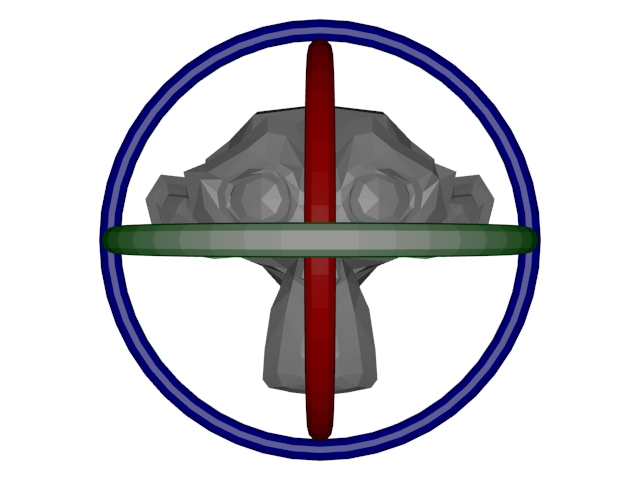
\includegraphics[scale=0.44]{figs_camaraypose/gimbal1}
				\label{fig: gimbal1}}
        \subfigure[]{
                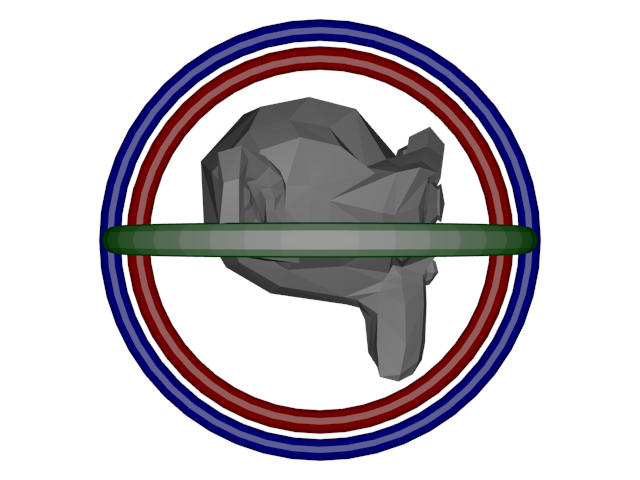
\includegraphics[scale=0.44]{figs_camaraypose/gimbal90y}
                \label{fig: gimbal90y}}
        
       \subfigure[]{
                
\includegraphics[scale=0.44]{figs_camaraypose/gimbal60x}
				\label{fig: gimbal60x}}
        \subfigure[]{
                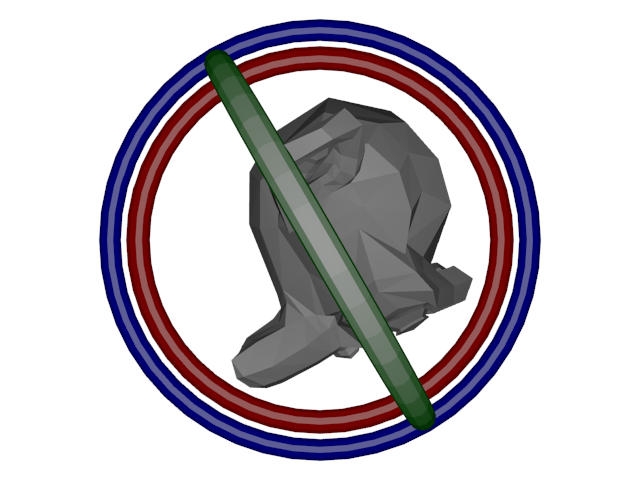
\includegraphics[scale=0.44]{figs_camaraypose/gimbal60z}
                \label{fig: gimbal60z}}
         \caption{Los ejes rojo, verde y azul, son los ejes $x$, $y$ y $z$. En \subref{fig: gimbal1} se ve la posici�n inicial. En \subref{fig: gimbal90y} se puede ver el eje $y$ rotado $90^\circ$. En \subref{fig: gimbal60x} se ve la rotaci�n seg�n $x$ de $60^\circ$ respecto a la posici�n de \subref{fig: gimbal90y}. En \subref{fig: gimbal60z} se ve la rotaci�n seg�n $z$ de $-60^\circ$ respecto a la posici�n de \subref{fig: gimbal90y}.}
\end{figure}

\subsection{Cuaternios}
Los cuaternios son una extensi�n a los n�meros reales, son generados a\~nadiendo las unidades imaginarias \textit{i}, \textit{j} y \textit{k}. Se cumple que $i^2 = j^2  = k^2 = -1$. Un n�mero cuaternio $q$ se expresa como $q = a + bi + cj +dk$. Tambi�n puede ser expresado como un escalar y un vector de 3 elementos $(a,\textbf{v})$. Una rotaci�n alrededor del versor $\omega$ un �ngulo $\theta$ se puede expresar como el n�mero cuaternio unidad
$$ q = \left(\cos\left(\frac{1}{2}\theta\right),\omega\sin\left(\frac{1}{2}\theta\right)\right)$$

Para rotar un punto 3D \textbf{M}, se representa como un cuaternio $p = (0,\textbf{M})$ y el punto $p'$ rotado se calcula como 
$$p' = q p \overline{q}.$$ 
El producto que se utiliza es el producto de cuaternios y $\overline{q} = \left(\cos\left(\frac{1}{2}\theta\right),-\omega\sin\left(\frac{1}{2}\theta\right)\right)$ es el cuaternio conjugado de $q$.

Esta representaci�n evita el problema del \textit{gimbal lock} pero tiene como contra que tiene un mayor  costo computacional. 






\bibliographystyle{unsrt}   
\bibliography{encuadro}  
\end{document}
